\documentclass[a4paper,12pt]{report}
\usepackage{graphicx}
\usepackage{titlesec}
\titleformat{\chapter}{}{}{0em}{\bf\LARGE}
\usepackage[utf8]{inputenc}

% Title Page
\title{Middle East Technical University\\Department of Physics\\PHYS222 Optics and Waves Laboratory\\\textbf{Experiment OW-10 Optical Activity\\Laboratory Report}}

\author{Oğuzhan ÖZCAN\\1852334\\\\Partner: İnci SAİM\\\\Teaching Assistant: Kamil ÇINAR}

\begin{document}
\maketitle
\tableofcontents
\listoffigures
\listoftables
\chapter{Theory}
Some substances have the ability to rotate the plane of polarization of light passing through  them. This phenomenon is known as optical activity. Note that in some textbooks this term also known as \textit{circular birefringence}. Optical activity was first observed in 1811 by French physicist Dominique F.J. Arago in the form of colours in sunlight that had passed along the optic axis of a quartz crystal placed between crossed polarizers [1]. Further experiments have done by Jean Baptiste Biot in 1812. Biot states that any material that causes to electrical field of an incident linear plane wave to appear to rotate is known as optically active. When a beam of linearly polarized light passed through the optically active medium, the light will emerge with its plane of polarization that turned through an angle which is proportional to the length of the path of the light through that medium. Then the amount of rotation per unit length of travel is called the \textit{specific rotatory power} which is denoted by $[\alpha]$ [2]. Biot also found that one must distinguish between right and left rotation. 
\begin{figure}[h]
\centering
\includegraphics[width=0.85\linewidth, height=0.30\textheight]{"optical system"}
\caption{Basic experiment in optical activity}
\label{fig:opticalsystem}
\end{figure}

Substances which cause the plane of polarization to rotate to the right or clockwise are called \textit{dextrorotatory} and  substances which cause the plane of polarization to rotate to the left counterclockwise are called \textit{levorotatory} [3]. To define the specific rotatory power assume that $n_{R}$ and $n_{L}$ denote the indices of refraction of the medium for right and left circularly polarized light. Then corresponding wave numbers should be $k_{R}=n_{R}\omega/c$ and $k_{L}=n_{L}\omega/c$. If we suppose that a beam of linearly polarized light travels a distance $L$ through the medium, we will have 
\begin{center}
	$\psi=\frac{1}{2}(k_{R}+k_{L})L$\\ 
$\theta=\frac{1}{2}(k_{R}-k_{L})L$ 
\end{center} 
where $\psi$ is the ellipticity which is obtained from the ratio of the minor and major axes of the ellipse. This equations represents a linearly polarized wave in which the direction of polarization is turned through an angle $\theta$ with respect to the original direction of polarization. From previous equations then we have 
\begin{center}
	$\theta=(n_{R}-n_{L})\frac{\omega L}{2c}$\\
$\theta=(n_{R}-n_{L})\frac{\pi L}{\lambda}$
\end{center}
where $\lambda$ is the wavelength in vacuum. By using these equations we can define specific rotatory power as a function of wavelength which is given by 
\begin{center}
	$[\alpha]=(n_{R}-n_{L})\frac{\pi}{\lambda}$
\end{center}
As we mentioned before ellipticity $\psi$ is another important quantity in optical activity which is very useful to define the circular dichroism [1]. To clarify the ellipticity let assume that $E_{R}$ is the electric field of right circular polarized light and $E_{L}$ is the electric field of left circular polarized light. Then  ellipticity shoul be 
\begin{center}
	$\psi=\tan^{-1}[\frac{(E_{R}-E_{L})}{(E_{R}-E_{L})}]$
\end{center}
When $E_{R}>E_{L}$, $\psi$ is positive which is correspond to a clockwise rotation of the electric field vector of the ellipticaly polarized light beam in a fixed plane. When we define this quantity with related to wavelength, path length and index, we would have 
\begin{center}
	$E_{l}=E_{0}$e$^{-2\pi n'l/\lambda}$
\end{center}
where $l$ is the related path length and $n'$ is the absorption index. Unit of specific rotatory power is \textbf{deg dm$^{-1}$ g$^{-1}$ mL}.\\\\
When we back to optical activity as a term, in chemistry this phenomena is known as \textit{optical isomerism}. If we give an example when an optically active complex is synthesized, a mixture of the two
optical isomers is obtained, such as the two $[Co(en)_{3}]^{3+}$ isomers in figure 1.2. The optical rotation of one isomer just cancels that of
the other [4]. In this sense we have faced with a new term which known as \textit{chirality}.    
\begin{figure}[h]
\centering
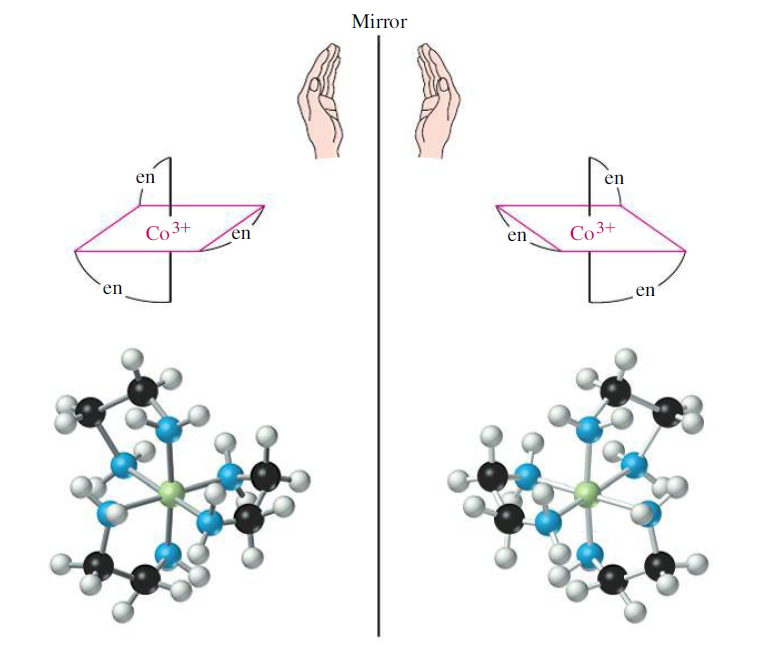
\includegraphics[width=0.50\linewidth, height=0.25\textheight]{isomerism}
\caption{Optical isomers}
\label{fig:isomerism}
\end{figure}
Chirality or handedness is a characteristic feature of living systems. Natural L-amino
acids and D-ribose exemplify the preference for one particular mirror image form,
called dextrorotary (D) and levorotary (L) enantiomeric configuration. Thus, an
asymmetric or chiral carbon atom is one around which four different substituents
can be arranged in left- or right-handed orientation. A chiral compound is present in
two mirror image molecules (enantiomers). Extant life depends on chiral homogeneity
for the structure and function of biopolymers [5].The most common feature in chiral molecules is a tetrahedral (i.e. sp$^{3}$-
hybridized) carbon atom with four different atoms or groups attached. Such
a carbon atom is called a chiral carbon or an asymmetric carbon. Chiral
molecules do not have a plane of symmetry [6]. When there are two or more atoms/groups that are the same, the carbon is
called achiral. Achiral molecules often have a plane of symmetry. If a
molecule can be divided by a plane into two equal halves that are mirror
images of each other, the plane is a plane of symmetry, and the molecule is not chiral. With achiral molecules, the compound and its mirror image are the same, i.e. they can be superimposed [7]. 



\chapter{Data and Results}
\begin{table}[h]
	\begin{center}
\begin{tabular}{|c|c|c|c|c|}
	\hline Solutions & $\theta_{1}$ & $\theta_{2}$ & $\theta_{3}$ & Average \\ 
	\hline Solution 1 & 104$^{\circ}$
	 & 102$^{\circ}$
	  & 104$^{\circ}$
	   & 103.34$^{\circ}$
	    \\ 
	\hline Solution 2 & 50$^{\circ}$
	 & 50$^{\circ}$
	  & 50$^{\circ}$
	   & 50$^{\circ}$
	    \\ 
	\hline Solution 3 & 30$^{\circ}$
	 & 30$^{\circ}$
	  & 32$^{\circ}$
	   & 30.67$^{\circ}$
	    \\ 
	\hline Solution 4 & 8$^{\circ}$
	 & 8$^{\circ}$
	  & 8$^{\circ}$
	   & 8$^{\circ}$
	    \\ 
	\hline 
\end{tabular} 
\end{center}
\caption{Rotation of Plane of Polarization}
\end{table}
\textbf{1. According to your measurements is the solution dextrorotatory or laevorotatory?}\\\\
In the chemistry literature, the medium is said to be dextrorotatory if the plane
of polarization rotates clockwise (positive angle of rotation), and levarotatory if
the plane of polarization rotates counterclockwise (negative angle of rotation), when
viewed towards the source of the light. Since we rotated plane of polarization as clockwise, we have \textbf{dextrorotatory} solution.\\\\
\textbf{2. Concentration of the tube $\#1$ is 1.01 g/mL. The error is given as $\pm$ 0.01 g/mL for concentration. The concentration of the enumerated solution is half of the preceding ones. The degree of $2^{\circ}$ may be taken as the error of angle measurements.}
\begin{table}[h]
	\begin{center}
\begin{tabular}{|c|c|}
	\hline Solutions & Concentration \\ 
	\hline Solution 1 & 1.01 g/mL \\ 
	\hline Solution 2 & 0.505 g/mL \\ 
	\hline Solution 3 & 0.2525 g/mL \\ 
	\hline Solution 4 & 0.12625 g/mL \\ 
	\hline 
\end{tabular} 
\end{center}
\caption{Concentrations of Solutions}
\end{table}
\\\\
\textbf{3. Plot the angle of rotation versus the concentaration graph.}\\\\
Please see graph paper.\\\\
\textbf{4. Using the graph find the rotation power $[\alpha]$ of the sugar molecules.}\\\\
Graph's equation is \textit{y=103.6x-1.0439}. In the angle of rotation versus concentration graph slope is correspond to rotation power $[\alpha]$. Thus in this graph slope is 103.6 which is our rotation power. Note that since unit of rotation power is deg dm$^{-1}$ g$^{-1}$ mL we have to divide 103.6 by 1 dm to reach the correct unit. If we calculate rotation power by using following equation
\begin{center}
{\large 	$[\alpha]=\frac{\alpha (deg)}{L (dm) C (g/mL)}$}
\end{center}
where $\alpha$ is observed rotation, $L$ is the path length (length of the tube) and $C$ is the concentration of solution. In the following calculations, $L$ is 1 dm, angle of rotation $\alpha$ can be obtained from Table 2.1 and related concentaritions can be obtained from Table 2.2.\\\\
For Solution $\#1$
\begin{center}
	$[\alpha_{1}]=\frac{103.34^{\circ}}{1dm\times1.01g/ml}$
\end{center}
\begin{center}
$[\alpha_{1}]=102.31$ deg dm$^{-1}$ g$^{-1}$ mL 
\end{center}
For Solution $\#2$
\begin{center}
	$[\alpha_{2}]=\frac{50^{\circ}}{1dm\times0.505g/ml}$
\end{center}
\begin{center}
	$[\alpha_{2}]=99.0$ deg dm$^{-1}$ g$^{-1}$ mL 
\end{center}
For Solution $\#3$
\begin{center}
	$[\alpha_{3}]=\frac{30.8^{\circ}}{1dm\times0.2525g/ml}$
\end{center}
\begin{center}
	$[\alpha_{3}]=121.98$ deg dm$^{-1}$ g$^{-1}$ mL 
\end{center}
For Solution $\#4$
\begin{center}
	$[\alpha_{4}]=\frac{8^{\circ}}{1dm\times0.12625g/ml}$
\end{center}
\begin{center}
	$[\alpha_{4}]=63.67$ deg dm$^{-1}$ g$^{-1}$ mL 
\end{center}


\chapter{Discussion and Conclusion}
\textbf{1.What are the possible errors in the experiment?}\\
There are some possible errors in the experiment. The first one is about the lazer. The lazer that used in laboratory was polarized. According to theory of optical activity light should be unpolarized. The second possible error was reflected light from wall. While doing experiment, sometimes it was hard to see light beam. The third one is about scaling. As mentioned in laboratory manual we have $2^{\circ}$ possible error in the angle measurement. The last possible error is about compound. Our solutions has corn based sugar and as we know sugar can crystallise and crystallisation may cause to diffraction. \\\\ 
\textbf{2.What kind of approximation did you take into consideration while you were obtaining the physical quantities and how do they affect your results?}\\
As we mentioned before angle measurement may have $2^{\circ}$ error. When we were reading angle scale we tried to collect best data. Before each solution we checked our lazer, polarizer and analyzer with a tube which contain water. The aim was set experiment setup to zero.\\\\   
\textbf{3.What discrepancies did you encounter between the calculated quantities and theoretical or literature values?}\\
We do not have certain discrepancies because our experimental results are very close to theoretical ones. When we look at the graph we can see that slope is almost same with theoretical value.\\\\ 
\textbf{4.What is your overall conclusion?}\\
In my opinion the experiment was successful because we observed good measurements. Applications of optics in chemistry are studied well.   
We have acceptable errors in our data.




















\chapter{Application}
\textbf{Polarimetry}\\
Polarimetry is a sensitive, nondestructive technique for measuring the optical activity exhibited by inorganic and organic compounds. A compound is considered to be optically active if linearly polarized light is rotated when passing through it. The amount of optical rotation is determined by the molecular structure and concentration of chiral molecules in the substance. Each optically active substance has its own specific rotation as defined in Biot's law. Historically, polarimetry was performed using an instrument where the extent of optical rotation is estimated by visual matching of the intensity of split fields. For this reason, the D-line of the sodium lamp at the visible wavelength of 589nm was most often employed. Specific rotation determined at the D-line is expressed by the symbol:
\begin{center}
	$[\alpha]=(25) [D]$ or $[\alpha]=(20) [D]$
\end{center}
and much of the data available are expressed in this form. Use of lower wavelengths, such as those available with the mercury lamp lines isolated by means of filters of maximum transmittance at approximately 578, 546, 436, 405, and 365nm in a photoelectric polarimeter, have been found to provide advantages in sensitivity with a consequent reduction in the concentration of the test compound. In general, the observed optical rotation at 436nm is about double and at 365nm about three times that at 589nm. Reduction in the concentration of the solute required for measurement may sometimes be accomplished by conversion of the substance under test to one that has a significantly higher optical rotation. Optical rotation is also affected by the solvent used for the measurement, and this is always specified.\\\\
The polarimetric method is a simple and accurate means for determination and investigation of structure in macro, semi-micro and micro analysis of expensive and non-duplicable samples. Polarimetry is employed in quality control, process control and research in the pharmaceutical, chemical, essential oil, flavor and food industries [8].

 
\chapter{References}
$[1]$ Barron, L. (2004).\textit{ Molecular Light Scattering And Pptical Activity} (2nd ed., pp. 2-6). Cambridge, UK: Cambridge University Press.\\\\
$[2]$ Fowles, G. (1989). \textit{Introduction to Modern Optics} (2nd ed., Dover ed., p. 185). New York: Dover Publications.\\\\
$[3]$ Kenyon, I. (2008). \textit{The Light Fantastic: A Modern Introduction to Classical and Quantum Optics} (p. 281). Oxford [England: Oxford University Press.\\\\
$[4]$ Petrucci, R. (2011). \textit{General Chemistry: Principles and Modern Applications} (10th ed., p. 1082). Toronto, Ont.: Pearson Canada.\\\\
$[5]$ Gel, R. (2011). \textit{Chirality and Life a Short Introduction to The Early Phases of Chemical Evolution} (p. 9). Berlin: Springer.\\\\
$[6]$ Sarker, S., \& Nahar, L. (2007). \textit{Chemistry for Pharmacy Students: General, Organic and Natural Product Chemistry} (p. 42). Chichester, England: John Wiley \& Sons.\\\\
$[7]$ Gschneidner, K. (2007). \textit{Handbook on the Physics and Chemistry of Rare Earths} (p. 273). Amsterdam: Elsevier.\\\\
$[8]$ Polarimetry Definitions, Fundementals, Applications for Industry. (n.d.). Retrieved March 31, 2015, from http://rudolphresearch.com/products/polari\\meters/polarimetry-definitions/
























































































\end{document}          
